% Template Matching is a general purpose method usually used for object
% recognition. A template is created for the sought object and an image is scanned
% with the template, calculating a matching cost for each possible position.

% Naively applying template matching to the barcode reading problem would not
% yield an interesting algorithm, because after choosing a scanline, reading is
% reduced to finding a barcode such that the 

Our reading method is taken from \cite{Gallo2011} and is based on matching
deformable templates to a 1D scanline obtained from the localization and
boundary detection steps.
From the previous steps, we get left and right boundary candidates as
positions on the image, as well as the best line from the LSD step, the height
of which we assume to be the height of the barcode.
Since there are no time restrictions, we now try all combinations of left and
right boundary candidates. For each left/right pair, we also try seven offsets
along the height of the barcode and for each offset, we try both possible
orientations (up/down). For example, if we get three left and three right
boundary candidates from the LSD Bound step, a total number of $3\cdot
3\cdot 7 \cdot 2=126$ different scanlines would be tried.

Let $p_l$ and $p_r$ denote the positions of the current left and right boundary
candidates. Since an EAN-13 barcode consists of 95 base widths, an initial
estimate of the base width is $w=\norm{p_l-p_r}/95$. Since the number of base
widths in each pattern (guard or digit) is known, we can calculate an initial
estimate of the offset along the scanline at which each pattern should begin. A
naive (non-deformable) template matching algorithm would now match a template
for each possible pattern (digits 0-9, types A,B and C) against the scanline,
scaled such that the base width is $w$, starting at the estimated offset.

However, there is an uncertainty associated with the estimates, $\Delta w$ for
the base width and $\Delta o$ for the offsets. These uncertainties are due to
inaccuracies of the boundary detection, kinks in the material, etc. For example,
if the perspective is skewed, the base width at the end of the barcode which is
closer to the camera might be larger than the base width at the farther end. In
our implementation we chose $\Delta o=3w$ and $\Delta w=2\Delta o/95$. Based on a distance measure between
templates and grey values on the scanline (for details see \cite{Gallo2011}), we calculate the matching probability for each possible
template at each position. We integrate over every offset and base width in the
ranges $[o-\Delta o, o+\Delta o]$ and $[w-\Delta w, w+\Delta w]$, scaling and translating the
templates appropriately along the scanline. In addition to the matching
probabilities, we calculate least squares estimates $(\bar{o}, \bar{w})$ for
offset and base width for each template.
To make the computation of the
integrals efficient, we use the method proposed by \citeauthor{Gallo2011}, which
is based on precalculating cells in $(o, w)$-space in which the distance between
template and scanline is constant.

% We define the overlap cost between the $j$-th and $(j+1)$-th template as
% \begin{equation*}
%  O_j 
% \end{equation*}
From the least squares estimates, the overlap between two templates at two
consecutive positions can be calculated.
Since the digits in the barcode don't overlap, the sequence of templates corresponding
to the true patterns in the barcode should have small overlap in addition to the
high individual matching probability. We use the dynamic programming scheme
proposed in \cite{Gallo2011} to determine the sequence of templates which
optimizes the matching and overlapping cost globally.

Finally, we calculate the first digit from the first six digit types (A or B).
If the digit types don't form a valid pattern as described in the standard, we
return a reading failure. If the check digit doesn't match, we return a failure
as well.

Our implementation  differs from the one described in \cite{Gallo2011} in the
following ways:
\begin{itemize}
\item We extended the method from UPC barcodes to EAN-13 barcodes.
\item Because there are no time constraints, we use a larger uncertainty
  $\Delta w$.
\item If a digit lies next to a guard pattern, we extend the template by the
  guard pattern's bars.
\end{itemize}

Since we try a large number of scanlines, the same barcode might be read
multiple times, or different scanlines might yield different barcode readings.
We choose the returned barcode reading by the minimal total matching cost as well as
favoring barcodes which have been read more often.
\begin{figure}[t]
\center
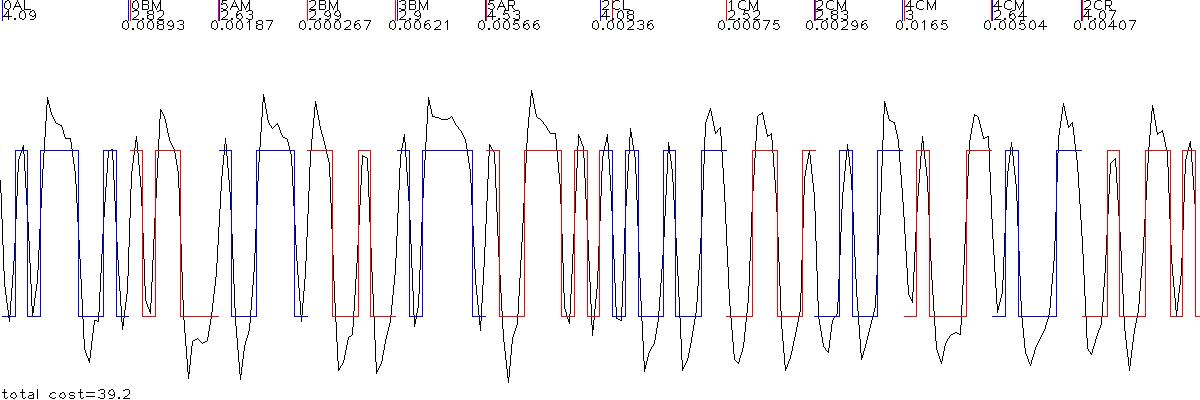
\includegraphics[width=\textwidth,natwidth=1200,natheight=400]{img/tmpl.jpg}
\caption{Successful reading with template matching. Templates shown in red and blue.}
\label{tmpl}
\end{figure}





% Let $S=\set{0A, 1A,\cdots 9A, 0B, \cdots, 9C}$ be the set of possible patterns.
% A base template for the pattern $s\in S$ is a function $\mm^s(x)$ as shown in
% FIGGGGGURE. The patterns from the EAN-13 standard are augmented by one bar of
% the The deformed template has been shifted by an offset $o$ and scaled
% by a base width $w$:
% \begin{equation*}
%  \mm^s_{o,w} (x)=\mm^s((x-o)/w)
% \end{equation*}
% For each position in the barcode and conditioned on a specific choice of $o$ and $w$, we
% can calculate the matching probability for a pattern $s\in S$ as
% \begin{equation*}
%  p_s(I\mid o,w) \propto e^{-D(I, \mm^s_{o,w})}\,,
% \end{equation*}
% where $I(n)$ represents the grey values of the current scanline. $D$ is a
% distance measure between the template and the scanline and is calculated
% pixel by pixel:
% \begin{equation*}
%   D(I, \mm^s_{o,w}) = \sum_{n=}
% \end{equation*}

%%% Local Variables:
%%% mode: latex
%%% TeX-master: "00Ausarbeitung.tex"
%%% End:
